\documentclass{article}
\usepackage{tikz}
\begin{document}
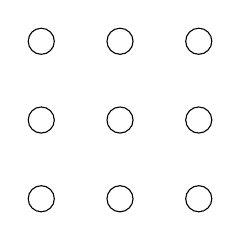
\begin{tikzpicture}
\node[shape=circle, draw=black] (0) at (2,0) {};
\node[shape=circle, draw=black] (1) at (0,1) {};
\node[shape=circle, draw=black] (2) at (0,2) {};
\node[shape=circle, draw=black] (3) at (1,2) {};
\node[shape=circle, draw=black] (4) at (1,1) {};
\node[shape=circle, draw=black] (5) at (2,2) {};
\node[shape=circle, draw=black] (6) at (1,0) {};
\node[shape=circle, draw=black] (7) at (2,1) {};
\node[shape=circle, draw=black] (8) at (0,0) {};
\end{tikzpicture}
\end{document}